% latex table generated in R 3.2.3 by xtable 1.8-0 package
% Mon Feb  8 22:09:15 2016
\begin{longtable}{lL{1.8cm}C{2cm}lcc}
\caption{Number of taxa with available discrete morphological data for mammalian orders at three taxonomic levels. The left vertical bar represents low coverage (\textless 25\%; coloured in blue); the right vertical bar represents high coverage (\textgreater 75\%; coloured in orange). Negative Net Relatedness Index (NRI) and Nearest Taxon Index (NTI) values indicate phylogenetic overdispersion; positive values indicate phylogenetic clustering. Significant NRI or NTI values are in bold. *p \textless 0.05; **p \textless 0.01; ***p \textless 0.001.
} \\ 

  \hline
Order & Taxonomic level & Proportion of taxa & Coverage & NRI & NTI \\ 
  \hline
  Mammalia (class) & family & 129/148 & 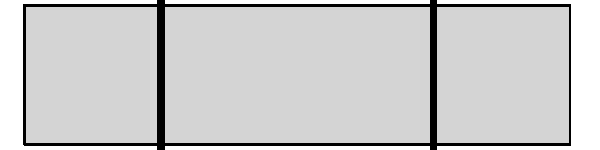
\includegraphics[width=0.20\linewidth, height=0.05\linewidth]{Table_figures_color/bar40.pdf} & -1.19 & 1.09 \\ 
  \textbf{Mammalia (class)} & \textbf{genus} & \textbf{517/1186} & 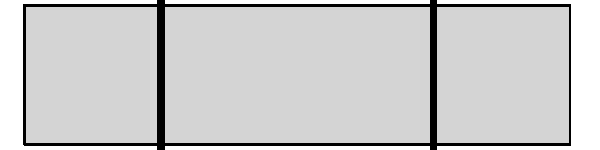
\includegraphics[width=0.20\linewidth, height=0.05\linewidth]{Table_figures_color/bar41.pdf} & \textbf{-5.19} & \textbf{3.71**} \\ 
  \textbf{Mammalia (class)} & \textbf{species} & \textbf{847/5017} & 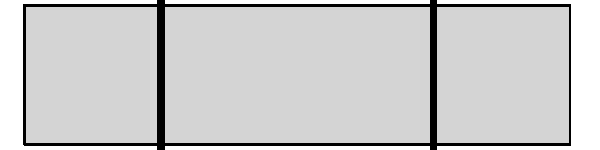
\includegraphics[width=0.20\linewidth, height=0.05\linewidth]{Table_figures_color/bar42.pdf} & \textbf{-7.75} & \textbf{3.54**} \\ 
  Afrosoricida & family & 2/2 & 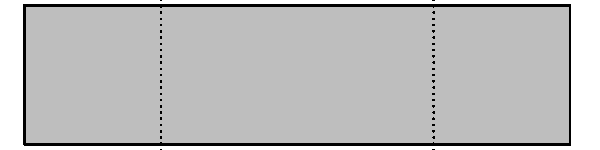
\includegraphics[width=0.20\linewidth, height=0.05\linewidth]{Table_figures_color/bar1.pdf} &   &   \\ 
  Afrosoricida & genus & 17/17 & 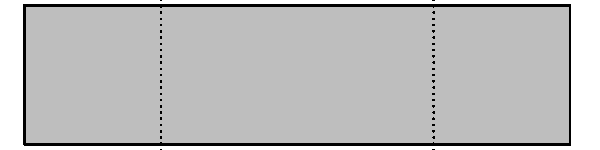
\includegraphics[width=0.20\linewidth, height=0.05\linewidth]{Table_figures_color/bar2.pdf} &   &   \\ 
  Afrosoricida & species & 23/42 & 
\includegraphics[width=0.20\linewidth, height=0.05\linewidth]{Table_figures_color/bar3.pdf} & 1.52 & 1.1 \\ 
  Carnivora & family & 14/15 & 
\includegraphics[width=0.20\linewidth, height=0.05\linewidth]{Table_figures_color/bar4.pdf} & 0.65 & 0.55 \\ 
  \textbf{Carnivora} & \textbf{genus} & \textbf{52/125} & 
\includegraphics[width=0.20\linewidth, height=0.05\linewidth]{Table_figures_color/bar5.pdf} & \textbf{4.27**} & \textbf{1.26} \\ 
  \textbf{Carnivora} & \textbf{species} & \textbf{75/283} & 
\includegraphics[width=0.20\linewidth, height=0.05\linewidth]{Table_figures_color/bar6.pdf} & \textbf{7.24**} & \textbf{0.8} \\ 
  Cetartiodactyla & family & 21/21 & 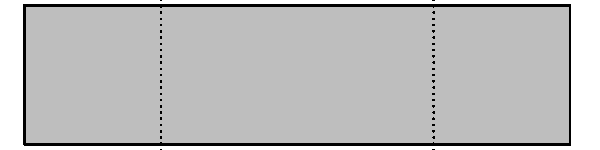
\includegraphics[width=0.20\linewidth, height=0.05\linewidth]{Table_figures_color/bar7.pdf} &   &   \\ 
  Cetartiodactyla & genus & 97/128 & 
\includegraphics[width=0.20\linewidth, height=0.05\linewidth]{Table_figures_color/bar8.pdf} & 0.7 & 1.28 \\ 
  \textbf{Cetartiodactyla} & \textbf{species} & \textbf{169/310} & 
\includegraphics[width=0.20\linewidth, height=0.05\linewidth]{Table_figures_color/bar9.pdf} & \textbf{1.82*} & \textbf{-0.24} \\ 
  Chiroptera & family & 15/18 & 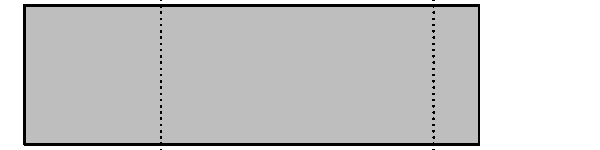
\includegraphics[width=0.20\linewidth, height=0.05\linewidth]{Table_figures_color/bar10.pdf} & -0.23 & 0.61 \\ 
  \textbf{Chiroptera} & \textbf{genus} & \textbf{92/202} & 
\includegraphics[width=0.20\linewidth, height=0.05\linewidth]{Table_figures_color/bar11.pdf} & \textbf{13.07**} & \textbf{0.99} \\ 
  \textbf{Chiroptera} & \textbf{species} & \textbf{214/1053} & 
\includegraphics[width=0.20\linewidth, height=0.05\linewidth]{Table_figures_color/bar12.pdf} & \textbf{9.21**} & \textbf{1.27} \\ 
  Cingulata & family & 1/1 & 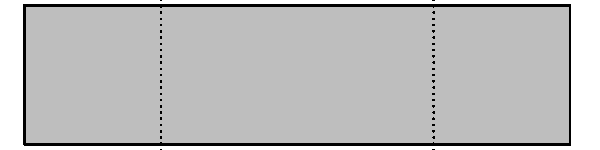
\includegraphics[width=0.20\linewidth, height=0.05\linewidth]{Table_figures_color/bar13.pdf} &   &   \\ 
  Cingulata & genus & 8/9 & 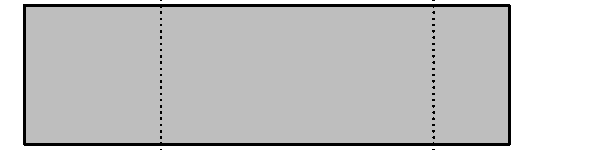
\includegraphics[width=0.20\linewidth, height=0.05\linewidth]{Table_figures_color/bar14.pdf} & 1.48 & -1.54 \\ 
  \textbf{Cingulata} & \textbf{species} & \textbf{9/29} & 
\includegraphics[width=0.20\linewidth, height=0.05\linewidth]{Table_figures_color/bar15.pdf} & \textbf{2.06*} & \textbf{0.2} \\ 
  Dasyuromorphia & family & 2/2 & 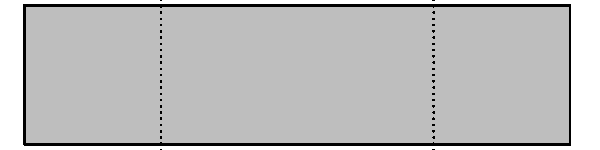
\includegraphics[width=0.20\linewidth, height=0.05\linewidth]{Table_figures_color/bar16.pdf} &   &   \\ 
  Dasyuromorphia & genus & 8/22 & 
\includegraphics[width=0.20\linewidth, height=0.05\linewidth]{Table_figures_color/bar17.pdf} & -0.78 & -1.06 \\ 
  Dasyuromorphia & species & 9/64 & 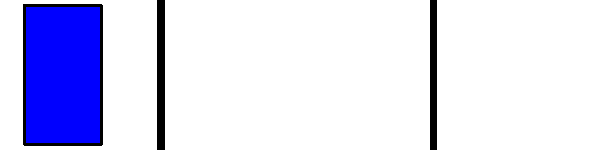
\includegraphics[width=0.20\linewidth, height=0.05\linewidth]{Table_figures_color/bar18.pdf} & -0.86 & -0.37 \\ 
  Dermoptera & family & 1/1 & 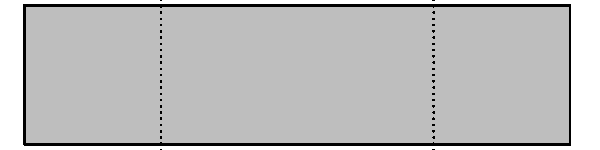
\includegraphics[width=0.20\linewidth, height=0.05\linewidth]{Table_figures_color/bar19.pdf} &   &   \\ 
  Dermoptera & genus & 1/2 & 
\includegraphics[width=0.20\linewidth, height=0.05\linewidth]{Table_figures_color/bar20.pdf} &   &   \\ 
  Dermoptera & species & 1/2 & 
\includegraphics[width=0.20\linewidth, height=0.05\linewidth]{Table_figures_color/bar21.pdf} &   &   \\ 
  Didelphimorphia & family & 1/1 & 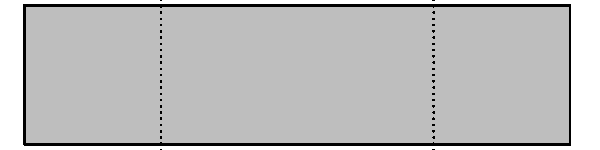
\includegraphics[width=0.20\linewidth, height=0.05\linewidth]{Table_figures_color/bar22.pdf} &   &   \\ 
  Didelphimorphia & genus & 16/16 & 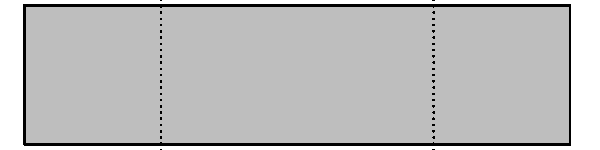
\includegraphics[width=0.20\linewidth, height=0.05\linewidth]{Table_figures_color/bar23.pdf} &   &   \\ 
  Didelphimorphia & species & 42/84 & 
\includegraphics[width=0.20\linewidth, height=0.05\linewidth]{Table_figures_color/bar24.pdf} & -1.61 & 0.12 \\ 
  Diprotodontia & family & 11/11 & 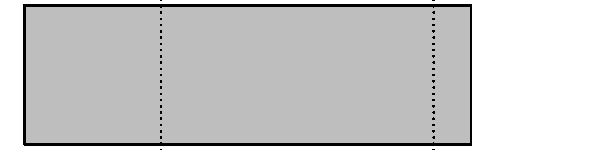
\includegraphics[width=0.20\linewidth, height=0.05\linewidth]{Table_figures_color/bar25.pdf} &   &   \\ 
  Diprotodontia & genus & 25/38 & 
\includegraphics[width=0.20\linewidth, height=0.05\linewidth]{Table_figures_color/bar26.pdf} & -1.15 & -1.33 \\ 
  Diprotodontia & species & 31/126 & 
\includegraphics[width=0.20\linewidth, height=0.05\linewidth]{Table_figures_color/bar27.pdf} & 0.44 & -1.79 \\ 
  Erinaceomorpha & family & 1/1 & 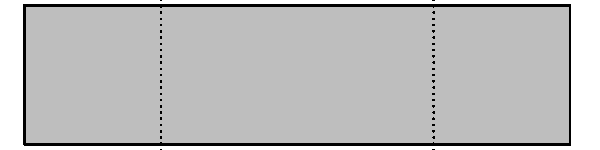
\includegraphics[width=0.20\linewidth, height=0.05\linewidth]{Table_figures_color/bar28.pdf} &   &   \\ 
  Erinaceomorpha & genus & 10/10 & 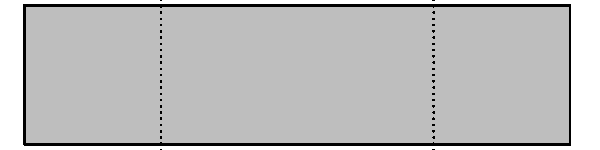
\includegraphics[width=0.20\linewidth, height=0.05\linewidth]{Table_figures_color/bar29.pdf} &   &   \\ 
  Erinaceomorpha & species & 21/22 & 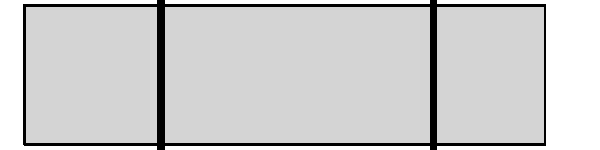
\includegraphics[width=0.20\linewidth, height=0.05\linewidth]{Table_figures_color/bar30.pdf} & -1.04 & -0.25 \\ 
  Hyracoidea & family & 1/1 & 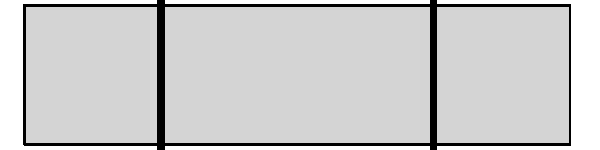
\includegraphics[width=0.20\linewidth, height=0.05\linewidth]{Table_figures_color/bar31.pdf} &   &   \\ 
  Hyracoidea & genus & 1/3 & 
\includegraphics[width=0.20\linewidth, height=0.05\linewidth]{Table_figures_color/bar32.pdf} &   &   \\ 
  Hyracoidea & species & 1/4 & 
\includegraphics[width=0.20\linewidth, height=0.05\linewidth]{Table_figures_color/bar33.pdf} &   &   \\ 
  Lagomorpha & family & 2/2 & 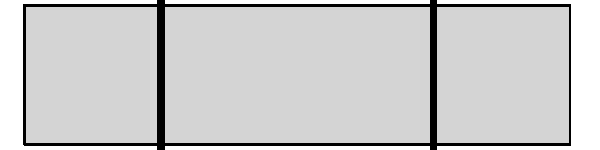
\includegraphics[width=0.20\linewidth, height=0.05\linewidth]{Table_figures_color/bar34.pdf} &   &   \\ 
  Lagomorpha & genus & 5/12 & 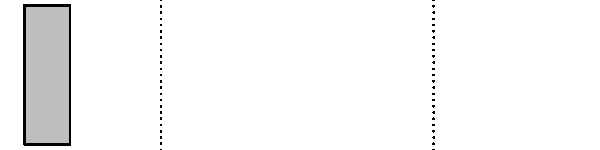
\includegraphics[width=0.20\linewidth, height=0.05\linewidth]{Table_figures_color/bar35.pdf} & -0.95 & -0.94 \\ 
  Lagomorpha & species & 12/86 & 
\includegraphics[width=0.20\linewidth, height=0.05\linewidth]{Table_figures_color/bar36.pdf} & -0.62 & -1.96 \\ 
  Macroscelidea & family & 1/1 & 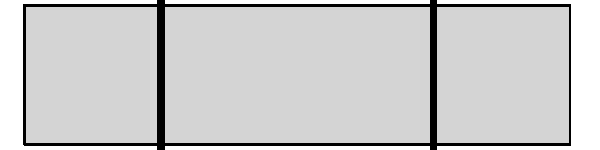
\includegraphics[width=0.20\linewidth, height=0.05\linewidth]{Table_figures_color/bar37.pdf} &   &   \\ 
  Macroscelidea & genus & 4/4 & 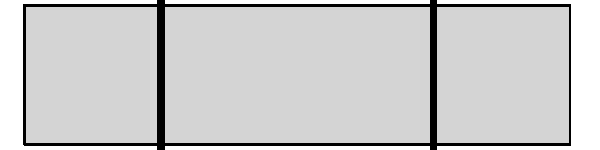
\includegraphics[width=0.20\linewidth, height=0.05\linewidth]{Table_figures_color/bar38.pdf} &   &   \\ 
  Macroscelidea & species & 12/15 & 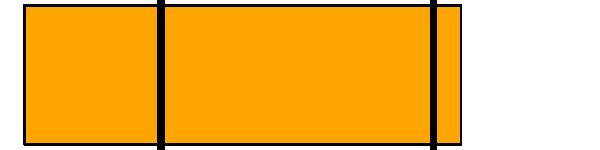
\includegraphics[width=0.20\linewidth, height=0.05\linewidth]{Table_figures_color/bar39.pdf} & -1.24 & -1.2 \\ 
  Microbiotheria & family & 1/1 & 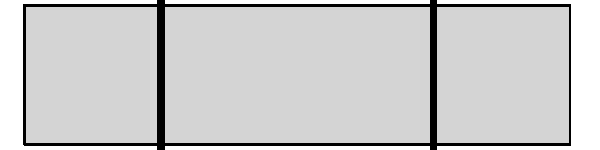
\includegraphics[width=0.20\linewidth, height=0.05\linewidth]{Table_figures_color/bar43.pdf} &   &   \\ 
  Microbiotheria & genus & 1/1 & 
\includegraphics[width=0.20\linewidth, height=0.05\linewidth]{Table_figures_color/bar44.pdf} &   &   \\ 
  Microbiotheria & species & 1/1 & 
\includegraphics[width=0.20\linewidth, height=0.05\linewidth]{Table_figures_color/bar45.pdf} &   &   \\ 
  Monotremata & family & 2/2 & 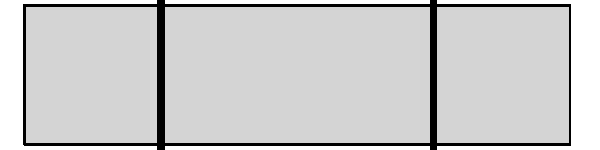
\includegraphics[width=0.20\linewidth, height=0.05\linewidth]{Table_figures_color/bar46.pdf} &   &   \\ 
  Monotremata & genus & 2/3 & 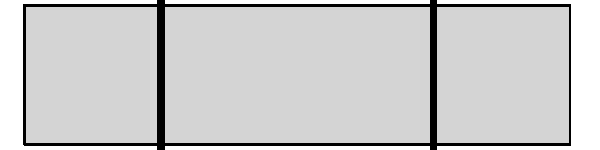
\includegraphics[width=0.20\linewidth, height=0.05\linewidth]{Table_figures_color/bar47.pdf} & -0.68 & -0.69 \\ 
  Monotremata & species & 2/4 & 
\includegraphics[width=0.20\linewidth, height=0.05\linewidth]{Table_figures_color/bar48.pdf} & -1.01 & -1 \\ 
  Notoryctemorphia & family & 1/1 & 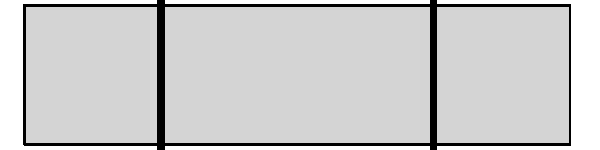
\includegraphics[width=0.20\linewidth, height=0.05\linewidth]{Table_figures_color/bar49.pdf} &   &   \\ 
  Notoryctemorphia & genus & 1/1 & 
\includegraphics[width=0.20\linewidth, height=0.05\linewidth]{Table_figures_color/bar50.pdf} &   &   \\ 
  Notoryctemorphia & species & 0/2 & \includegraphics[width=0.20\linewidth, height=0.05\linewidth]{Table_figures_color/bar51.pdf} &   &   \\ 
  Paucituberculata & family & 1/1 & \includegraphics[width=0.20\linewidth, height=0.05\linewidth]{Table_figures_color/bar52.pdf} &   &   \\ 
  Paucituberculata & genus & 3/3 & \includegraphics[width=0.20\linewidth, height=0.05\linewidth]{Table_figures_color/bar53.pdf} &   &   \\ 
  Paucituberculata & species & 5/5 & \includegraphics[width=0.20\linewidth, height=0.05\linewidth]{Table_figures_color/bar54.pdf} &   &   \\ 
  Peramelemorphia & family & 2/2 & \includegraphics[width=0.20\linewidth, height=0.05\linewidth]{Table_figures_color/bar55.pdf} &   &   \\ 
  Peramelemorphia & genus & 7/7 & \includegraphics[width=0.20\linewidth, height=0.05\linewidth]{Table_figures_color/bar56.pdf} &   &   \\ 
  Peramelemorphia & species & 16/18 & \includegraphics[width=0.20\linewidth, height=0.05\linewidth]{Table_figures_color/bar57.pdf} & -0.14 & 0.91 \\ 
  Perissodactyla & family & 3/3 & \includegraphics[width=0.20\linewidth, height=0.05\linewidth]{Table_figures_color/bar58.pdf} &   &   \\ 
  Perissodactyla & genus & 6/6 & \includegraphics[width=0.20\linewidth, height=0.05\linewidth]{Table_figures_color/bar59.pdf} &   &   \\ 
  Perissodactyla & species & 10/16 & \includegraphics[width=0.20\linewidth, height=0.05\linewidth]{Table_figures_color/bar60.pdf} & -0.1 & -2.77 \\ 
  Pholidota & family & 1/1 & \includegraphics[width=0.20\linewidth, height=0.05\linewidth]{Table_figures_color/bar61.pdf} &   &   \\ 
  Pholidota & genus & 1/1 & \includegraphics[width=0.20\linewidth, height=0.05\linewidth]{Table_figures_color/bar62.pdf} &   &   \\ 
  Pholidota & species & 4/8 & \includegraphics[width=0.20\linewidth, height=0.05\linewidth]{Table_figures_color/bar63.pdf} & 1.14 & 0.97 \\ 
  Pilosa & family & 4/5 & \includegraphics[width=0.20\linewidth, height=0.05\linewidth]{Table_figures_color/bar64.pdf} & 2.01 & 1.96 \\ 
  Pilosa & genus & 4/5 & \includegraphics[width=0.20\linewidth, height=0.05\linewidth]{Table_figures_color/bar65.pdf} & -0.91 & 0.36 \\ 
  \textbf{Pilosa} & \textbf{species} & \textbf{5/29} & \includegraphics[width=0.20\linewidth, height=0.05\linewidth]{Table_figures_color/bar66.pdf} & \textbf{1.18} & \textbf{2.35**} \\ 
  Primates & family & 15/15 & \includegraphics[width=0.20\linewidth, height=0.05\linewidth]{Table_figures_color/bar67.pdf} &   &   \\ 
  Primates & genus & 48/68 & \includegraphics[width=0.20\linewidth, height=0.05\linewidth]{Table_figures_color/bar68.pdf} & -0.37 & -1.39 \\ 
  Primates & species & 64/351 & \includegraphics[width=0.20\linewidth, height=0.05\linewidth]{Table_figures_color/bar69.pdf} & -0.66 & -1.4 \\ 
  Proboscidea & family & 1/1 & \includegraphics[width=0.20\linewidth, height=0.05\linewidth]{Table_figures_color/bar70.pdf} &   &   \\ 
  Proboscidea & genus & 2/2 & \includegraphics[width=0.20\linewidth, height=0.05\linewidth]{Table_figures_color/bar71.pdf} &   &   \\ 
  Proboscidea & species & 2/3 & \includegraphics[width=0.20\linewidth, height=0.05\linewidth]{Table_figures_color/bar72.pdf} & -0.67 & -0.72 \\ 
  Rodentia & family & 18/32 & \includegraphics[width=0.20\linewidth, height=0.05\linewidth]{Table_figures_color/bar73.pdf} & 0.66 & -0.95 \\ 
  \textbf{Rodentia} & \textbf{genus} & \textbf{82/450} & \includegraphics[width=0.20\linewidth, height=0.05\linewidth]{Table_figures_color/bar74.pdf} & \textbf{-1.81} & \textbf{1.7*} \\ 
  \textbf{Rodentia} & \textbf{species} & \textbf{90/2094} & \includegraphics[width=0.20\linewidth, height=0.05\linewidth]{Table_figures_color/bar75.pdf} & \textbf{2.66**} & \textbf{2.36**} \\ 
  Scandentia & family & 2/2 & \includegraphics[width=0.20\linewidth, height=0.05\linewidth]{Table_figures_color/bar76.pdf} &   &   \\ 
  Scandentia & genus & 2/5 & \includegraphics[width=0.20\linewidth, height=0.05\linewidth]{Table_figures_color/bar77.pdf} & -0.77 & -0.76 \\ 
  Scandentia & species & 3/20 & \includegraphics[width=0.20\linewidth, height=0.05\linewidth]{Table_figures_color/bar78.pdf} & -2 & -0.8 \\ 
  Sirenia & family & 2/2 & \includegraphics[width=0.20\linewidth, height=0.05\linewidth]{Table_figures_color/bar79.pdf} &   &   \\ 
  Sirenia & genus & 2/2 & \includegraphics[width=0.20\linewidth, height=0.05\linewidth]{Table_figures_color/bar80.pdf} &   &   \\ 
  Sirenia & species & 4/4 & \includegraphics[width=0.20\linewidth, height=0.05\linewidth]{Table_figures_color/bar81.pdf} &   &   \\ 
  Soricomorpha & family & 3/4 & \includegraphics[width=0.20\linewidth, height=0.05\linewidth]{Table_figures_color/bar82.pdf} & -0.98 & -0.97 \\ 
  \textbf{Soricomorpha} & \textbf{genus} & \textbf{19/43} & \includegraphics[width=0.20\linewidth, height=0.05\linewidth]{Table_figures_color/bar83.pdf} & \textbf{7.07**} & \textbf{2.64**} \\ 
  \textbf{Soricomorpha} & \textbf{species} & \textbf{21/392} & \includegraphics[width=0.20\linewidth, height=0.05\linewidth]{Table_figures_color/bar84.pdf} & \textbf{10.17**} & \textbf{3.36**} \\ 
  Tubulidentata & family & 1/1 & \includegraphics[width=0.20\linewidth, height=0.05\linewidth]{Table_figures_color/bar85.pdf} &   &   \\ 
  Tubulidentata & genus & 1/1 & \includegraphics[width=0.20\linewidth, height=0.05\linewidth]{Table_figures_color/bar86.pdf} &   &   \\ 
  Tubulidentata & species & 1/1 & \includegraphics[width=0.20\linewidth, height=0.05\linewidth]{Table_figures_color/bar87.pdf} &   &   \\ 
   \hline
\hline
\label{Table_results}
\end{longtable}
